\title{Assignment 2 Report} % Title, modify to the name of experiment
\author{Yang Hongmeng}% Author, modify to your name
\date{\today}% Date, Modify to the DATE of EXPERIMENT


 \documentclass[12pt]{article}
\usepackage{graphicx}
\usepackage{booktabs}
 \usepackage{makecell}
 \usepackage{float}
 \newcommand{\diff}{\,\mathrm{d}}
\usepackage[margin=1in]{geometry}
\usepackage{fancyhdr}
\pagestyle{fancy}
\usepackage{extarrows}
\usepackage{breqn}
\usepackage[colorlinks,linkcolor=blue]{hyperref}
\newcommand{\N}{\mathbb{N}}
\newcommand{\Z}{\mathbb{Z}}
\newcommand{\trans}{^{\mathrm T}}
\usepackage{amssymb}
\usepackage[table]{xcolor}
\usepackage{bm}
\usepackage{array}
\usepackage{mathtools}
\usepackage[english]{babel}
\usepackage{natbib}
\usepackage{url}
\usepackage[utf8x]{inputenc}
\usepackage{amsmath}
\usepackage{graphicx}
\graphicspath{{images/}}
\usepackage{parskip}
\usepackage{fancyhdr}
\usepackage{vmargin}
\usepackage[font={bf, footnotesize}, textfont=md]{caption}
\usepackage{amsmath,amsthm,amssymb}


\newenvironment{theorem}[2][Theorem]{\begin{trivlist}
\item[\hskip \labelsep {\bfseries #1}\hskip \labelsep {\bfseries #2.}]}{\end{trivlist}}
\newenvironment{lemma}[2][Lemma]{\begin{trivlist}
\item[\hskip \labelsep {\bfseries #1}\hskip \labelsep {\bfseries #2.}]}{\end{trivlist}}
\newenvironment{exercise}[2][Exercise]{\begin{trivlist}
\item[\hskip \labelsep {\bfseries #1}\hskip \labelsep {\bfseries #2.}]}{\end{trivlist}}
\newenvironment{reflection}[2][Reflection]{\begin{trivlist}
\item[\hskip \labelsep {\bfseries #1}\hskip \labelsep {\bfseries #2.}]}{\end{trivlist}}
\newenvironment{proposition}[2][Proposition]{\begin{trivlist}
\item[\hskip \labelsep {\bfseries #1}\hskip \labelsep {\bfseries #2.}]}{\end{trivlist}}
\newenvironment{corollary}[2][Corollary]{\begin{trivlist}
\item[\hskip \labelsep {\bfseries #1}\hskip \labelsep {\bfseries #2.}]}{\end{trivlist}}
\DeclareMathOperator{\tr}{tr}
\DeclareMathOperator{\rank}{rank}
\DeclareMathOperator{\Span}{span}
\DeclareMathOperator{\row}{row}
\DeclareMathOperator{\col}{col}
\DeclareMathOperator{\range}{range}
\DeclarePairedDelimiterX{\inp}[2]{\langle}{\rangle}{#1, #2}
\DeclareMathOperator{\Proj}{Proj}
\DeclareMathOperator{\trace}{trace}
\newcommand{\Her}{^{\mathrm H}}
\DeclareMathOperator{\diag}{diag}
\makeatletter 
    \newcommand\fcaption{\def\@captype{table}\caption}
\makeatother
\setmarginsrb{3 cm}{2.5 cm}{3 cm}{2.5 cm}{1 cm}{1.5 cm}{1 cm}{1.5 cm}


\makeatletter
\let\thetitle\@title
\let\theauthor\@author
\let\thedate\@date
\makeatother

\pagestyle{fancy}
\fancyhf{}
\rhead{\theauthor}
\lhead{\thetitle}
\cfoot{\thepage}

\begin{document}

\begin{titlepage}
    \centering
    \vspace*{0.5 cm}
    
\includegraphics[scale = 0.75,width=6cm]{CUHK}\\[1.0 cm]   % University Logo
    \textsc{\large The Chinese University of Hong Kong, Shenzhen}\\[2.0 cm] 
    \textsc{\Large ECE4016}\\[0.5 cm] 
    \textsc{\large Computer Network}\\[0.5 cm]               % Course Name
    \rule{\linewidth}{0.2 mm} \\[0.4 cm]
    { \huge \bfseries \thetitle}\\
    \rule{\linewidth}{0.2 mm} \\[1.5 cm]
    
    \begin{minipage}{0.4\textwidth}
        \begin{flushleft} \large
            \emph{Author:}\\
            \theauthor
            \end{flushleft}
    \end{minipage}~
    \begin{minipage}{0.4\textwidth}
            \begin{flushleft} \large
            \emph{Student Number:} \\
             119010378  % Modify to your student number
        \end{flushleft}
    \end{minipage}\\[2 cm]
    {\large \thedate}\\[2 cm]
 
    \vfill
    
\end{titlepage}
\tableofcontents
\pagebreak
\rmfamily

\newpage
\section{Introduction}

In this assignment, I implement ABR algorithm by following the paper “Probe and adapt: Rate adaptation for HTTP video streaming at scale. (2014)”. Before introducing my implementation detail, I will introduce the background here.

Adaptive bitrate streaming (ABR) is a method for improving streaming over HTTP networks. The term “bitrate” refers to how quickly data travels across a network and is often used to describe an Internet connection’s speed. In this algorithm, the video steam would be segmented into several chunks. The server would also packet and send each chunk with different bitrate one time. 

However, the Internet environment changes all the time. Therefore, in order to make sure the quality of video and the experience of client, the client side server would choose which bitrate version of video chunk would be download according to current Internet condition.

Most of algorithm focus on how to make both video quality and the download speed good for client to use. The final target is to make the video quality as high as possible and the flow of video as fluent as possible.

In this report, I will show how conventional approach solve this problem and how I optimize this algorithm.

The detailed implementation methods and explanation are shown below.
\section{Algorithm implementation}

\subsection{Theoretical implementation}

The conventional approach has three steps:

First step is estimating the current bandwidth according to last time throughput. According to the given data, we can directly get the previous time throughput. 

The second step is smoothing the estimated bandwidth by utilizing the smooth function.

The last step is returning the bitrate by quantize the smoothed bandwidth.

\subsection{Actual implementation}

In my implementation, the first step is to get the available bitrate the next chunk can use. According to the previous given example code we can use “R\_i” to store the available bitrate. “R\_i” is a list which elements are pairs of theoretical bitrate and actual available bitrate. R\_i[i][0] is the string form of theoretical bitrate. In the experiment are 500000, 1000000 and 5000000. Additionally, R\_i[i][1] is the integer form of actual bitrate which depends on the Internet condition of that time.

At the same time, I use a variable named “xn” to be the estimated bandwidth. According to the algorithm of conventional approach the estimated bandwidth is equal to the previous time throughput. Therefore, the estimated bandwidth can directly get from the input.

The second step is to smooth the estimated bandwidth. I used two methods here: linear regression and EWMA smoother.

First, linear regression. This kind of smooth bandwidth is just for trying. I used all previous estimated bandwidth and chunk number to got a line and used the value of corresponding chunk number to get smoothed bandwidth. However, the problem of this kind of smooth is that if there is a huge drop of the throughput in recent several chunk, the line would give a relatively low value of smoothed bandwidth because considering those low point. Therefore, it may cause the bad performance in some cases.

Second, EWMA smoother. According to the equation given by the paper, the EWMA has a better performance after conducting those experiment. EWMA smoother utilizes the relationship of previous smoothed bandwidth, current estimated bandwidth and the time between current download operation and previous one to get a smoothed bandwidth.

~\\
\centerline {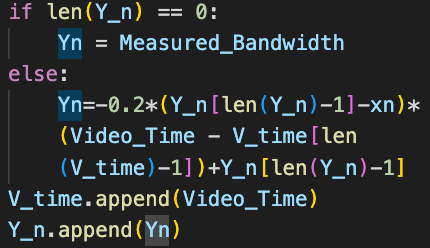
\includegraphics[scale = 1, width=6.2cm]{smooth}}
\centerline{\textbf {Figure 1: Smooth the estimated bandwidth}}

The third step is to quantize the smoothed bandwidth. In order to quantize the smoothed bandwidth, we should first get two boundary. The first boundary is named “R\_up” which is the actual bitrate of low boundary which is the maximu value of bitrate less than 0.85 smoothed bandwidth. 0.85 is default value which is given by the paper. The second boundary is named “R\_down” which is the actual bitrate of high boundary which is the maximu value of bitrate less than smoothed bandwidth.

~\\
\centerline {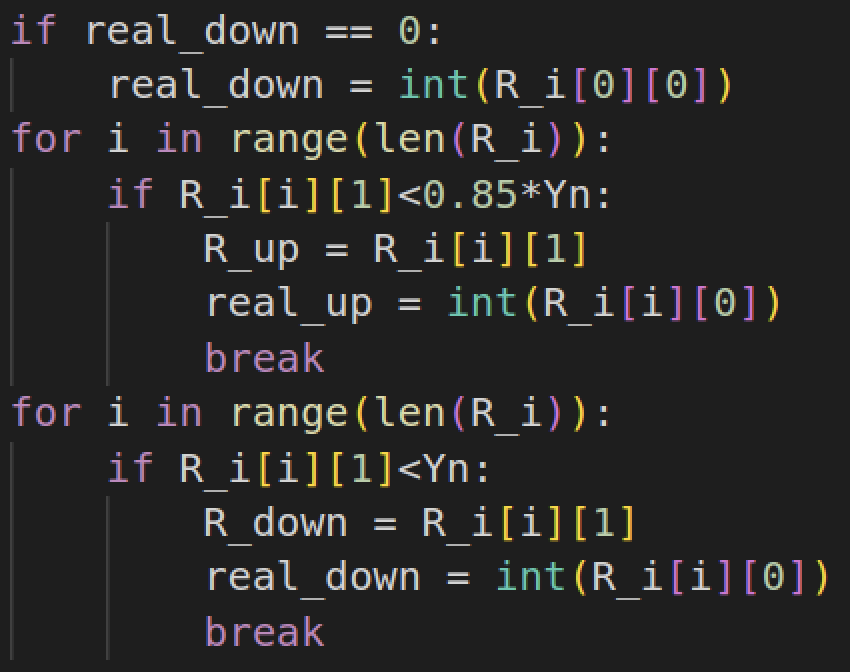
\includegraphics[scale = 1, width=6.2cm]{quan1}}
\centerline{\textbf {Figure 2: Dead-zone Quantizer step 1}}

Next step is using these two boundary and the previous bitrate to choose bitrate for next chunk. If the previous bitrate is smaller than “R\_up” then the bitrate is equal to corresponding theoretical bitrate of “R\_up”. If the bitrate is greater or equal to “R\_up” and smaller than “R\_down”, then the bitrate is equal to previous bitrate. Otherwise, the birtate is equal to corresponding theoretical bitrate of “R\_down”.

~\\
\centerline {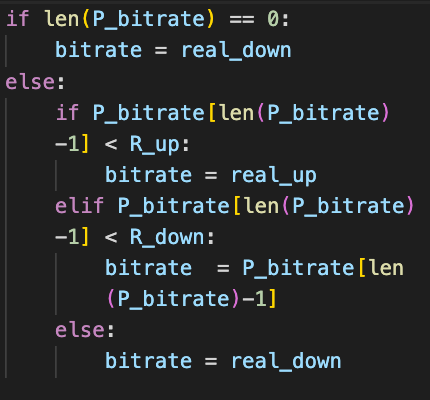
\includegraphics[scale = 1, width=6.2cm]{quan2}}
\centerline{\textbf {Figure 3: Dead-zone Quantizer step 2}}

\section{Result Analysis}

Compared with given example, my implementation algorithm has higher score on first two experiments and equal score of the third and last experiments. However, the given example has better performance on the fourth and fifth experiments. After doing the experiments, I found that the theoretical birtate and actual available bitrate has huge gap. Therefore, it would be better to check this kind of gap in order to get better performance. After I implement this method, all experiments have better or equal performance than the given example.

\section{Evaluation}

The performance of this algorithm has its own strength on estimating the next round bandwidth, which can help to choose next bitrate for user side server and control both download time and video quality. However, when the actual available bitrate has big gap with the theoretical bitrate, the performance of this algorithm is not good enough. After adding the comparison of smoothed estimated bandwidth and the theoretical bitrate, the performance increases. Additionally, the smooth function may also have optimization approach.

\section{Appendix}

\textbf {Additionally, I do not want my code used in the future or public, thank you in advanced.} And the following two figures show the grade result of two versions of my implementation.

~\\
\centerline {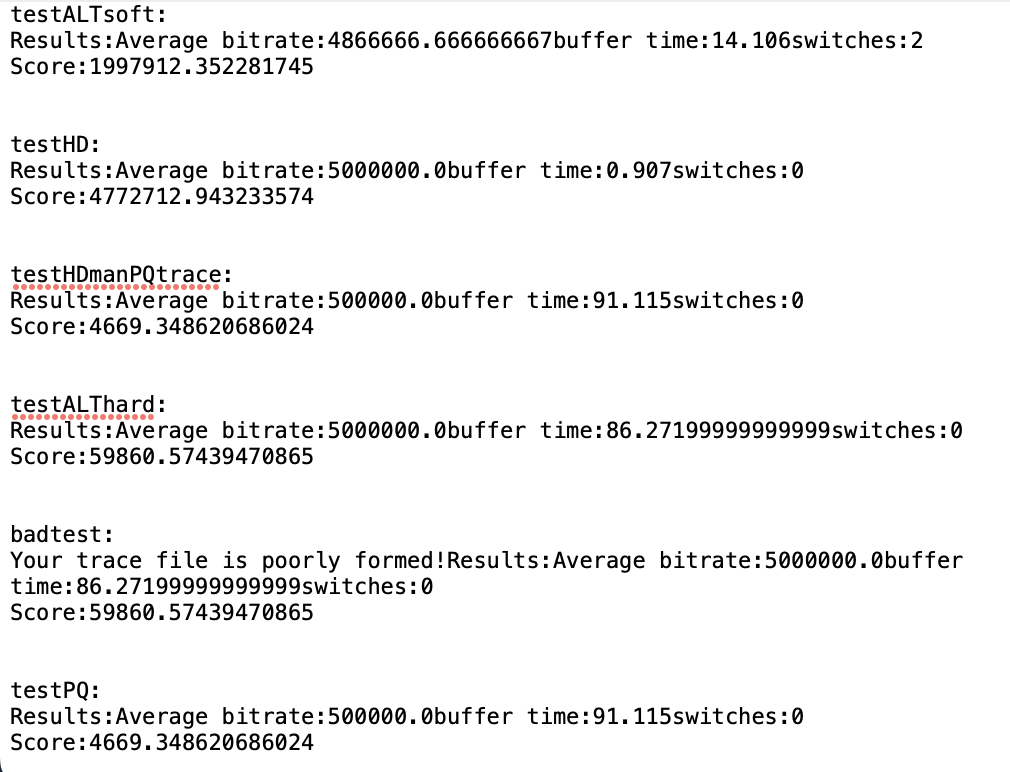
\includegraphics[scale = 1, width=10cm]{imp1}}
\centerline{\textbf {Figure 4: Test result without optimization}}

~\\
\centerline {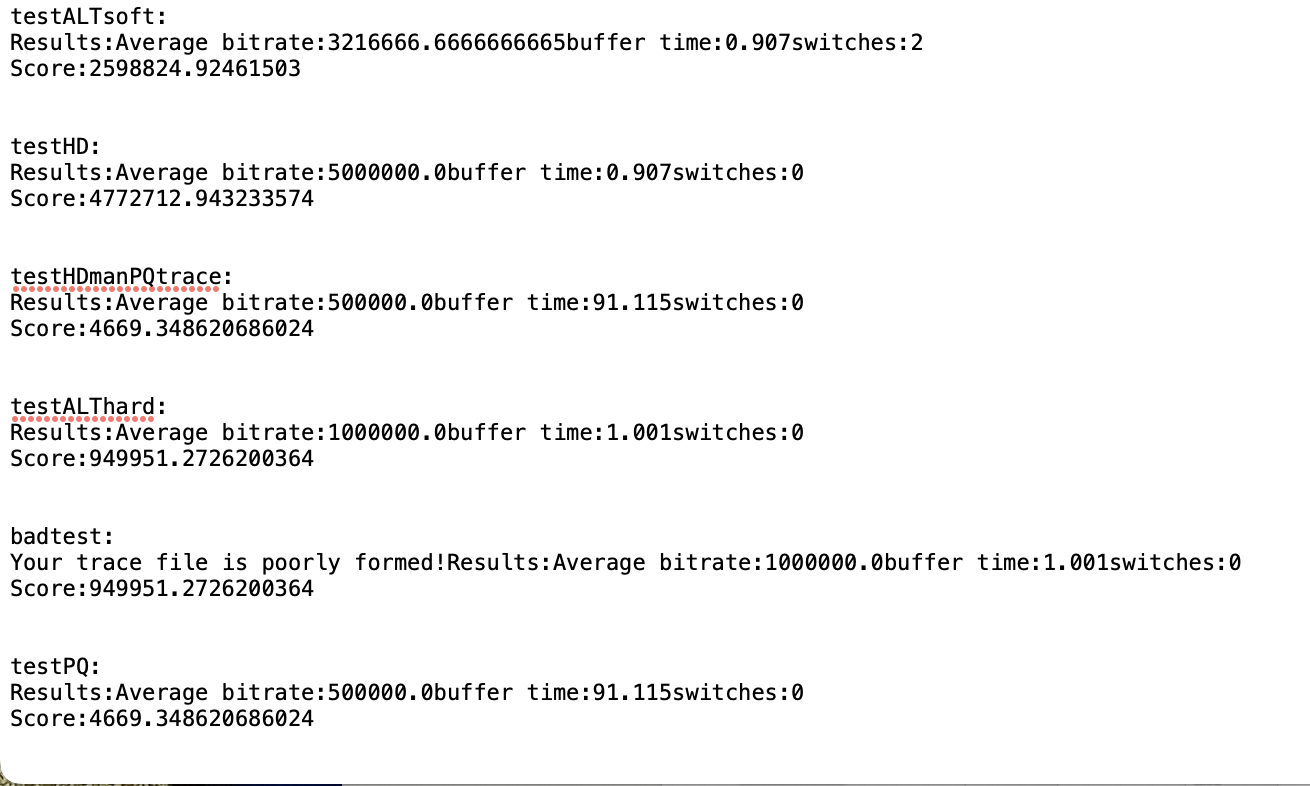
\includegraphics[scale = 1, width=14cm]{imp2}}
\centerline{\textbf {Figure 5: Test result with optimization}}

\end{document}
